\section{Einleitung}
Durch das Projekt NISABA\footnote{https://nisaba.dm.hs-furtwangen.de/} und der Veranstaltung Bildverarbeitung und Computergrafik im Studiengang Medieninformatik Master im Sommersemester 2021 sind 3D-Modelle der Kasernengebäude des Lyautey- und Mangin-Geländes entstanden. Um die fertigen 3D Modelle für jeden zugänglich und auf moderner Weise präsentieren zu können, wird in dieser Master-Arbeit eine Augmented Reality Anwendung für Smartphone und Tablet Geräte entwickelt.

Diese Forschungsarbeit beschäftigt sich mit der Entwicklung einer Augmented Reality \acrshort{ar} Anwendung. Durch genaues Tracking und eine realistische Darstellung der Gebäude durch wetterspezifische Belichtung, Schattierung und Spiegelung soll eine hohe Immersion erschaffen. In der Anwendung werden die 3D-Objekte in der Größendarstellung 1:1 über das Videobild der Kamera gelegt und der Nutzer kann vor Ort das Gebäude in Echtzeit ein- und ausblenden lassen. Dafür wird der Begriff \textit{world-scale Augmented Reality} herangezogen. Bekannte Beispiele sind das AR Spiel Pokemon GO\footnote{https://pokemongolive.com/de/} oder auch Anwendungen für Googles Holo Lens\footnote{https://www.microsoft.com/de-de/hololens}. Viele AR Anwendungen finden dabei in einem Raum oder in einem kleinen Radius statt, sodass die Umgebung einfach getrackt werden kann.

Eine wesentliche Rolle bei der Immersion in AR spielt das Tracking, bei dem kontinuierlich die Positions- und Rotationsdaten des Endgeräts erfasst werden. Es gibt mehrere Verfahren, um die Position und Orientierung der Kamera relativ zur Umgebung zu bestimmen. Im begrenzten Räumen ist das Tracking durch einheitlichere Belichtung und vorhandenen Kanten und Flächen mit kamerabasierten Tracking Methoden gut umsetzbar. Im Freien kann das Tracking je nach Umgebung Probleme bereiten. Schwierigkeiten entstehen durch unterschiedliche Lichtverhältnisse und dem größeren Suchraum. Hinzu kommt, dass durch die große Distanz zwischen Kamera und virtuellem Objekt die Platzierung des 3D-Modells bereits durch kleine Bewegung der Kamera stark von der korrekten Position abweicht. Das Objekt erscheint nicht homogen in der realen Welt, wodurch die Immersion beeinträchtigt wird.

Klassischerweise wird bei AR im Freien GPS und die Neigungs- und Beschleunigungssensoren der Smartphones genutzt, um die Kameraposition und -orientierung zu ermitteln. Wie Platinsky und seine Koautoren\cite{platinsky} bereits erörtert ist die GPS Lokalisierung insbesondere in Städten mit Störfaktoren wie Gebäuden oder Vegetation ungenau. Deshalb wird in dieser Arbeit auf Methoden eingegangen, um die Genauigkeit der Position und der Orientierung der Kamera im Freien zu verbessern.

Um die Immersion bei der Nutzung der App zu steigern, werden die Wetterbedingungen bei der Darstellung der 3D-Modelle berücksichtigt. So sollen die Fassaden bei regnerischem Wetter dunkler und gegebenenfalls spiegelnd dargestellt werden. Die Schattierungen sollen sich anpassen, indem bei hartem Licht (z.B. durch starke Sonneneinstrahlung) auch harte Schatten und bei weichem Licht (z.B. bei einer dichten Wolkendecke) weiche Schatten dargestellt werden.

\section{Forschungsstand}
Augmented Reality ist ein nachgefragtes Thema und wird in unterschiedlichen Bereichen wie Industrie, Medizin oder in der Computerspiel-Branche untersucht\cite{Sudirman}\cite{Santi}\cite{Huang}. Es gilt Probleme zu lösen, die sowohl Hardware als auch Software betreffen. Die Hardwareentwicklung betrifft dabei hauptsächlich die Mobilität bei der Nutzung. Beispielsweise funktioniert die HTC Vive nur mit einem Computer, der mit einem Kabel am Headset verbunden ist. Die Microsoft Holo Lens hingegen benötigt eine gute Internetverbindung über Wi-Fi. In der Software ist es eine Herausforderung aus den vielfältigen Software-Paketen eigene AR Anwendungen zu entwickeln. Nicht jede Software Bibliothek ist miteinander kompatibel, sodass die Entwicklung eine lange Einarbeitungszeit benötigt\cite*[Vgl.][]{Santi}.

Ein weiteres Problem in der Nutzung von AR ist die Beleuchtung der Umgebung. In Fabriken oder Lagern ist es dunkel und Lichter kommen aus verschiedenen Richtungen, während es im Freien die Wetterbedingungen wie starke Sonne oder Wolken, die störende Schatten verursachen, zu beachten gilt. Die unterschiedlichen Lichtverhältnisse rufen Ungenauigkeiten z.B. beim Tracking hervor.

\subsection{Tracking}
Der Begriff Tracking beschreibt die kontinuierliche Verfolgung von Positions- und Rotationsdaten, die von Eingabegeräten (z.B. VR Controller) oder Sensoren (z.B. \textit{Inertial Measurement Units} (Gyroskop und Beschleunigungssensoren)) erfasst werden. Die Bewegung eines starren Körpers kann \glqq durch die Angabe von sechs Werten (drei Koordinaten als Position und drei Winkel zur Beschreibung der Orientierung) für jeden Zeitschritt spezifiziert werden\grqq{}\cite*[Dörner (2019) S.119f.]{doerner}. 

Die Werte für die Position und Orientierung für ein Objekt werden als \textit{Freiheitsgrade (engl. Degrees of Freedom – DOF)} bezeichnet. Beim Tracking ist es das Ziel, die sechs Freiheitsgrade
für die Translation und Rotation der Kamera zu bestimmen bzw. zu schätzen\cite{doerner}. Es gibt zwei Tracking Systeme. Beim \textit{Inside-Out-Tracking} befinden sich Sensoren im Objekt, das getrackt werden soll, während beim \textit{Outside-In-Tracking} sich die Sensorik in der Umgebung befinden und das Objekt von außen getrackt wird. In dieser Arbeit wird ein Inside-Out-Tracking verwendet, da sich die Sensorik im Smartphone bzw. Tablet befinden.

\subsubsection{Koordinatensysteme}
Um eine Bestimmung bzw. Schätzung der Translationen und Rotationen durchzuführen, können zwei Koordinatensysteme herangezogen werden. Ein Kamerakoordinatensystem und ein Objektkoordinatensystem, womit die relativen Transformationen zwischen den Koordinatensystemen bestimmt werden können. Weiterhin gibt es die Möglichkeit, dass für alle Objekte im Raum ein Koordinatensystem (Weltkoordinatensystem) verwendet wird. Voraussetzung für das Tracking ist, dass die Transformationen zwischen den Objekten bekannt sind. Dann kann die Transformation zwischen der Kamera und das Weltkoordinatensystem geschätzt werden. Sind einzelne Transformationen von Objekten im Weltkoordinatensystem nicht bekannt, kann es auch Mischformen geben Zitat \cite*[Dörner (2019) S.124f.]{doerner}.

\subsection{Kamera-basiertes Tracking}
Kamera-basiertes Tracking nutzt Informationen zu Objekten aus dem Video Datenstrom, um die relative Position und Orientierung der Objekte zur Kamera zu bestimmen. Hartley und Zisserman bezeichnen diese als \textit(extrinsische Kameraparameter) \cite*[Hartley, Zisserman (2003) S.156]{hartleyzisserman}. Für das Kamera-basierte Tracking wird zwischen Marker-basierten und Marker-less Tracking unterschieden.

Beim Marker-basierten Tracking werden schwarz-weiß Marker (sogenannte Kanji und Hiro Marker) (Verweis) mit einfachen geometrischen Formen platziert und erkannt, sodass diese als als Orientierungshilfen fungieren. Eine Anwendung von NGIN-Mobility arbeitet mit Markern, die auf dem Boden platziert werden können \footnote{https://www.logistik-watchblog.de/startups/1479-insider-navigation-ar-loesung-lagerhalle.html}. Da die Marker in dauerhaft in der Umgebung platziert werden müssen, ist die Trackingmöglichkeit für die Nutzung im Freien ungeeignet.

Die zweite Möglichkeit erfasst über Algorithmen der Computer Vision Merkmale in der realen Umgebung. Diese Art wird als \textit{marker-less AR} bezeichnet. Merkmale können geometribasiert sein (z.B. Kanten, Formen wie Vierecke) oder es werden Detektoren wie z.B. \textit{SIFT (engl. Scale Invariant Feature Transform)}\cite{lowe_sift} oder \textit{SURF (engl. Scale Invariant Feature Transform)}\cite{bay_surf} verwendet. Auch die aus der Robotertechnik bekannte \textit{SLAM (engl. Simultaneous Localization and Mapping)}\cite{slam1} \cite{slam2} Methode wird genutzt. Dabei werden entweder kamerabasiert (Visual SLAM) nach Merkmalen gesucht oder es kommen Sensoren zur Generierung von Tiefeninformationen zum Einsatz, z.B. Kinect \footnote{https://developer.microsoft.com/de-de/windows/kinect/} oder \textit{LIDAR-Sensoren (engl. light detection and ranging)}\cite{liu_lai_lang}. Vorteil dieser Methode ist, dass gleichzeitig eine 3D-Karte des Raumes generiert wird, die immer wieder zur Positions- und Rotationsbestimmung verwendet werden kann.

\subsubsection{GPS Tracking}
Im Außenbereich wird bei AR auch GPS für das Tracking herangezogen. Dabei sind Positionsabweichungen von bis zu 10 Metern möglich, sodass eine genaue Bestimmung der extrinsischen Kameraparameter beeinträchtigt wird. Um die Tracking-Genauigkeit zu erhöhen, gibt es mehrere Methoden. \textit{DGPS (engl. Differential GPS)} verbessert GPS-Signale, indem es ein Korrektursignal durch eine ortsfeste Referenzstation mit bekannter Lokalisierung berechnet. Da es in Deutschland lediglich acht solcher Stationen gibt und einige Anbieter nur kommerziell die Daten bereitstellen, ist diese Methode nicht für diese Arbeit geeignet\footnote{https://www.heise.de/newsticker/meldung/Differential-GPS-und-WLAN-RTT-Praezise-Ortung-mit-Android-P-4046935.html} \footnote{Liste von DGPS-Sendern: https://www.ndblist.info/datamodes/worldDGPSdatabase.pdf}. Eine weitere bekannte Möglichkeit bietet \textit{SBAS (engl. Satellite Based Augmentation System)}, bei dem mehrere geostationäre Satelliten das GPS Signal auf bis zu einem Meter Genauigkeit zu verbessern \cite*{doerner}.

Platinsky und seine Koautoren\cite{platinsky} erstellen für ein besseres Tracking bei fehlender GPS Genauigkeit ein 3D-Modell der Umgebung. Bei der anschließenden AR Nutzung in diesem Gebiet wird auf dem Smartphone SLAM betrieben. Die Daten vom Smartphone werden mit der 3D-Karte verglichen, um ein genaueres Tracking durchzuführen. Ein ähnliches System wäre für die Anwendung in dieser Arbeit denkbar, da eine große Datenmenge von Bildern des Geländes vorhanden ist. Über Structure from Motion Methoden, kann mit den Bildern eine große 3D-Karte erstellt werden.

\begin{figure}[h]
    \centering
    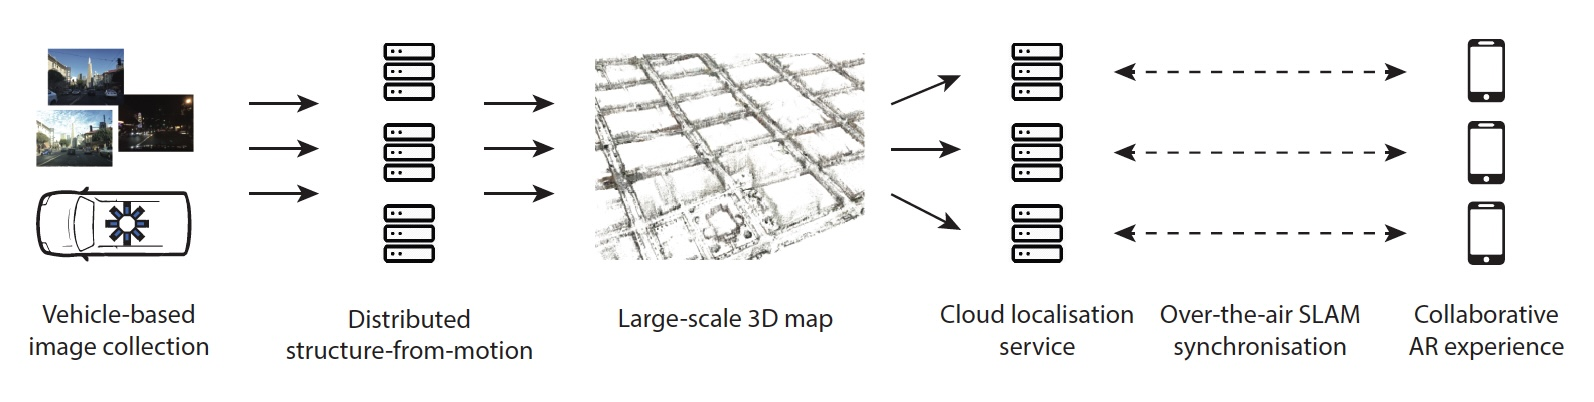
\includegraphics[width=\textwidth]{platinsky.jpg}
    \caption{Das Grundprinzip der Methode von Platinsky.}
    \label{fig:PlatinskyPrinzip}
\end{figure}

\subsection{Software Entwicklung}
Für Augmented Reality Anwendungen gibt es im Smartphone und Tablet Bereich mehrere Softwarepakete (\textit{SDK (engl. Software Development Kit)}. Die bekanntesten sind ARKit von Apple, das nur auf iOS Endgeräten läuft und ARCore von Google, das für Android Endgeräte entwickelt wird.\footnote{https://developer.apple.com/augmented-reality/} \footnote{https://developers.google.com/ar} Andere SDK's wie Vuforia\footnote{https://www.ptc.com/en/products/vuforia}, Wikitude\footnote{https://www.wikitude.com/}, ARToolKit\footnote{http://www.hitl.washington.edu/artoolkit/} oder Lightship\footnote{https://lightship.dev/} sind unabhängig vom Endgerät nutzbar.  

\section{Fragestellungen und Methodik}
Für die Entwicklung der AR Anwendung können die vorgestellten SDK's genutzt werden. Diese haben Vor- und Nachteile, die in dieser Arbeit erörtert werden, um daraus die passende SDK für dieses Projekt auszuwählen. Die Methode von Platinsky und seinen Koautoren\cite{platinsky}, in der das Tracking durch eine vorgefertigte 3D-Karte der Stadt verbessert wird, wird in dieser Arbeit weiter untersucht. Im Beispiel von Platinsky ist die GPS Genauigkeit durch die hohen Gebäude in der Großstadt stark beeinträchtigt. Das Gelände in Villingen befindet sich am Stadtrand und die Gebäude könnten keinen großen Einfluss auf die GPS Genauigkeit haben. Daher wird untersucht, ob der Mehraufwand, der durch die Erstellung der 3D Map und des SLAM Systems über eine Cloud entsteht, für eine mittelgroße Stadt sinnvoll ist. Hierfür wird die GPS Genauigkeit mit und ohne dieser Methode gemessen und miteinander verglichen.

Hinzu kommt die Frage, wie detailreich die 3D-Karte und die SLAM Daten des Smartphones für ein genaues Tracking sein müssen. Ein Problem der Methode ist, dass eine konstante Verbindung zum Internet bestehen muss, um die SLAM Daten mit der 3D-Karte zu vergleichen. Die 4G Verbindung war nicht ausreichend schnell \cite*[][sinngemäß aus]{platinsky}. Um an diesem Problem anzuknüpfen, wird untersucht, wie stark die Qualität der 3D-Karte reduziert werden kann, ohne die Vorteile beim Tracking zu verlieren. Eine Optimierung der Dateigröße der 3D-Karte wird im Paper zwar erwähnt, jedoch nicht umgesetzt. So wird in dieser Arbeit ein Experiment durchgeführt, bei der drei Qualitätsstufen (Hohe Details, mittlere Details, grobe Details) auf die GPS Genauigkeit untersucht werden. 

Je nachdem wie die Ergebnisse der Experimente ausgehen, ist es für die Anwendung sinnvoll dem Nutzer zwei Möglichkeiten anzubieten: Eine hohe Tracking Genauigkeit bei hohem Datenverbrauch und eine möglicherweise geringe Tracking Genauigkeit, bei dem diese Methode nicht genutzt wird.
